\documentclass[11pt,oneside,a4paper]{article}
%\usepackage{ucs}
\usepackage{url}
\usepackage{hyperref}
\usepackage[pdftex]{graphicx}
\usepackage{textcomp}
\usepackage[utf8]{inputenc}
\usepackage[finnish]{babel}
\usepackage[T1]{fontenc}
\author{Jari Koskinen, Hansi Keijonen, Eero Laine}
\title{Ohjelmointikielten periaatteet 2013}




\begin{document}
% kirjoita nimiö
\maketitle

\pagebreak

\tableofcontents

\pagebreak

\section{D ohjelmointikieli}
D on kehitetty korjaamaan C ja C++ kielten puutteita ja samalla siihen on lisätty paljon ominaisuuksia, joiden ansiosta...
\subsection{Yleistä}
D kielessä on ominaisuuksia plaaplaa...
\begin{itemize}
\item Automaattinen roskienkeruu
\item Vahva tyypitys
\item Käännös natiivikoodiksi
\item Rinnakkaisuuden tuki
\end{itemize}
Lisää kielestä plaaplaa...

\section{Erlang ohjelmointikieli}
Erlang on funktionaalinen kieli, joka on tarkoitettu alunperin puhelinkeskusten ohjelmointiin. Tästä syystä kieli tukee hyvin rinnakkaisuutta...
\subsection{Yleistä}
blaablaa
\section{Kielten alkiorakenteen vertailu}
\subsection{Tietotyypit}
D on vahvasti tyypitetty kieli...
Seuraavat tietotyypit ovat tuettuna:
\begin{itemize}
\item Int
\item Double
\item Char
\item ...
\end{itemize}
\subsection{Tunnukset}
...
\subsection{Varatut sanat, avainsanat}
...
...
\subsection{Literaalivakiot}
...
...
\subsection{Erottimet, sisennykset, rivinvaihdot}
...
...
\subsection{Esimerkkejä ohjelmakoodista}
...
...
\subsection{Ratkaisujen vertailua}
...
...
\section{Kielten syntaksi}
\subsection{Rakenne}
Näin tulostetaan Hello World!
\begin{verbatim}
import std.stdio;

void main() {
 writeln("Hello World!");
}
\end{verbatim}
C-kielestä tuttu tapa on mahdollinen...

\begin{verbatim}
import std.stdio;

void main() {
  for(int i=0; i<10; i++) {
    writeln("Rivi: ", i);
  }
}
\end{verbatim}
Iteraatio voidaan tehdä myös seuraavasti:
\begin{verbatim}
import std.stdio;

void main() {
  foreach(i; 0 .. 10) {
    writeln("Rivi: ", i);
  }
}
\end{verbatim}

ja tuloste näyttää kuvan \ref{konsoli1} mukaiselta.
\begin{figure}[tbh]
%\begin{figure}[tbh] t= top, b = bottom, h=here
\begin{center}
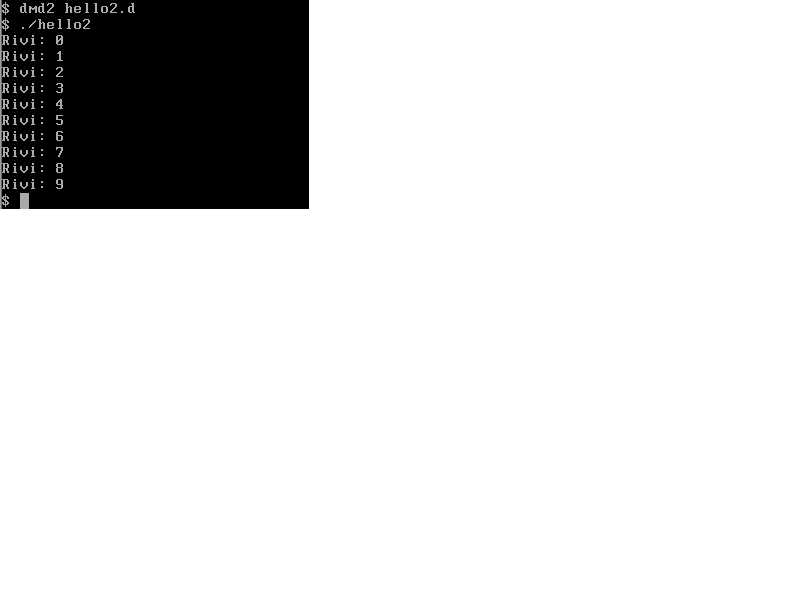
\includegraphics[width=1.0\textwidth]{konsoli1.jpg}
%\rotatebox{90}{\includegraphics[scale=.75]{esimerkki.pdf}}
\caption{Tuloste konsolilla}
\label{konsoli1}
\end{center}
\end{figure}

\section{Yhtenveto}
Yhteenvetona todettakoon, että D ja Erlang poikkeavat toisistaan...
\end{document}